\chapter{Implementation}
\label{cha:implementation}

Section 3 describes global requirements and the design of the authentication and authorization framework. This section now explains how the IdP of the \emph{device cloud} has been implemented, in a so-called User Directory.

\section{Components}
As a first step, the model implemented must be introduced. As said in the previous section, the model of the \emph{device cloud} encompasses at least the different Principals and the so-called consumer profile. The other components of the model, like the Request model (a Client sends a request to the User Directory by serializing a Request object) or the result of a request (the RequestResult model) are not required for the understanding of the framework and will therefore not be presented.

As shown in Fig. \ref{fig:principals}, all the entities of the \emph{device cloud} derive from a generic abstract Entity class, which contains global attributes like EntityOperator (already discussed in section \ref{03_authorizing}) or EntityType (i.e. Operator, Consumer, etc) and a generic ID. The Principals and the consumer profile classes will then extend this generic abstract Entity class, specifying at the same time the class of the generic field ID.

A Consumer could for instance be defined as an Entity whose ID is a String (like an email), whereas an Operator as an entity whose ID is a UID (Unique Identifier, i.e. a Long type). Both would still extend the Entity class and offer the same functionalities.

\subsection{Principals}
A Principal is defined as an entity, which inherits from the interfaces PrincipalEntity, ConfigurableEntity and AttachmentEntity, as one can see in Tab. \ref{tab:02_entities}, and whose ID is a PrincipalIdentifier. The PrincipalIdentifier class is a wrapper around a String identifier, which allows for various types of identifiers (GUID, email, alias) and offers conversion and type verification capabilities (a Globally unique identifier GUID or a UID should be a Long, an email should respect a certain format, etc).

Since a principal can be authenticated, it contains a \textit{secret} attribute, like a password, and a certificate (SSL authentication is required by the design). Attachments can be added (one could attach the certificate of the principal as a file for example) and a configuration (set of key value pairs) can also be defined.

This abstract class is then extended into the Consumer, Vendor, Operator, and Aggregator classes. These classes then define the appropriate EntityType and the attributes introduced in the previous sections (A ProtocolURI for the Operators for example). If required, they also implement the Location Tagged Entity Interface, with which the location of a Principal can be retrieved.

\begin{figure}[!hpbt]
	\centering
	\caption{Principal model}
	\label{fig:principals}
	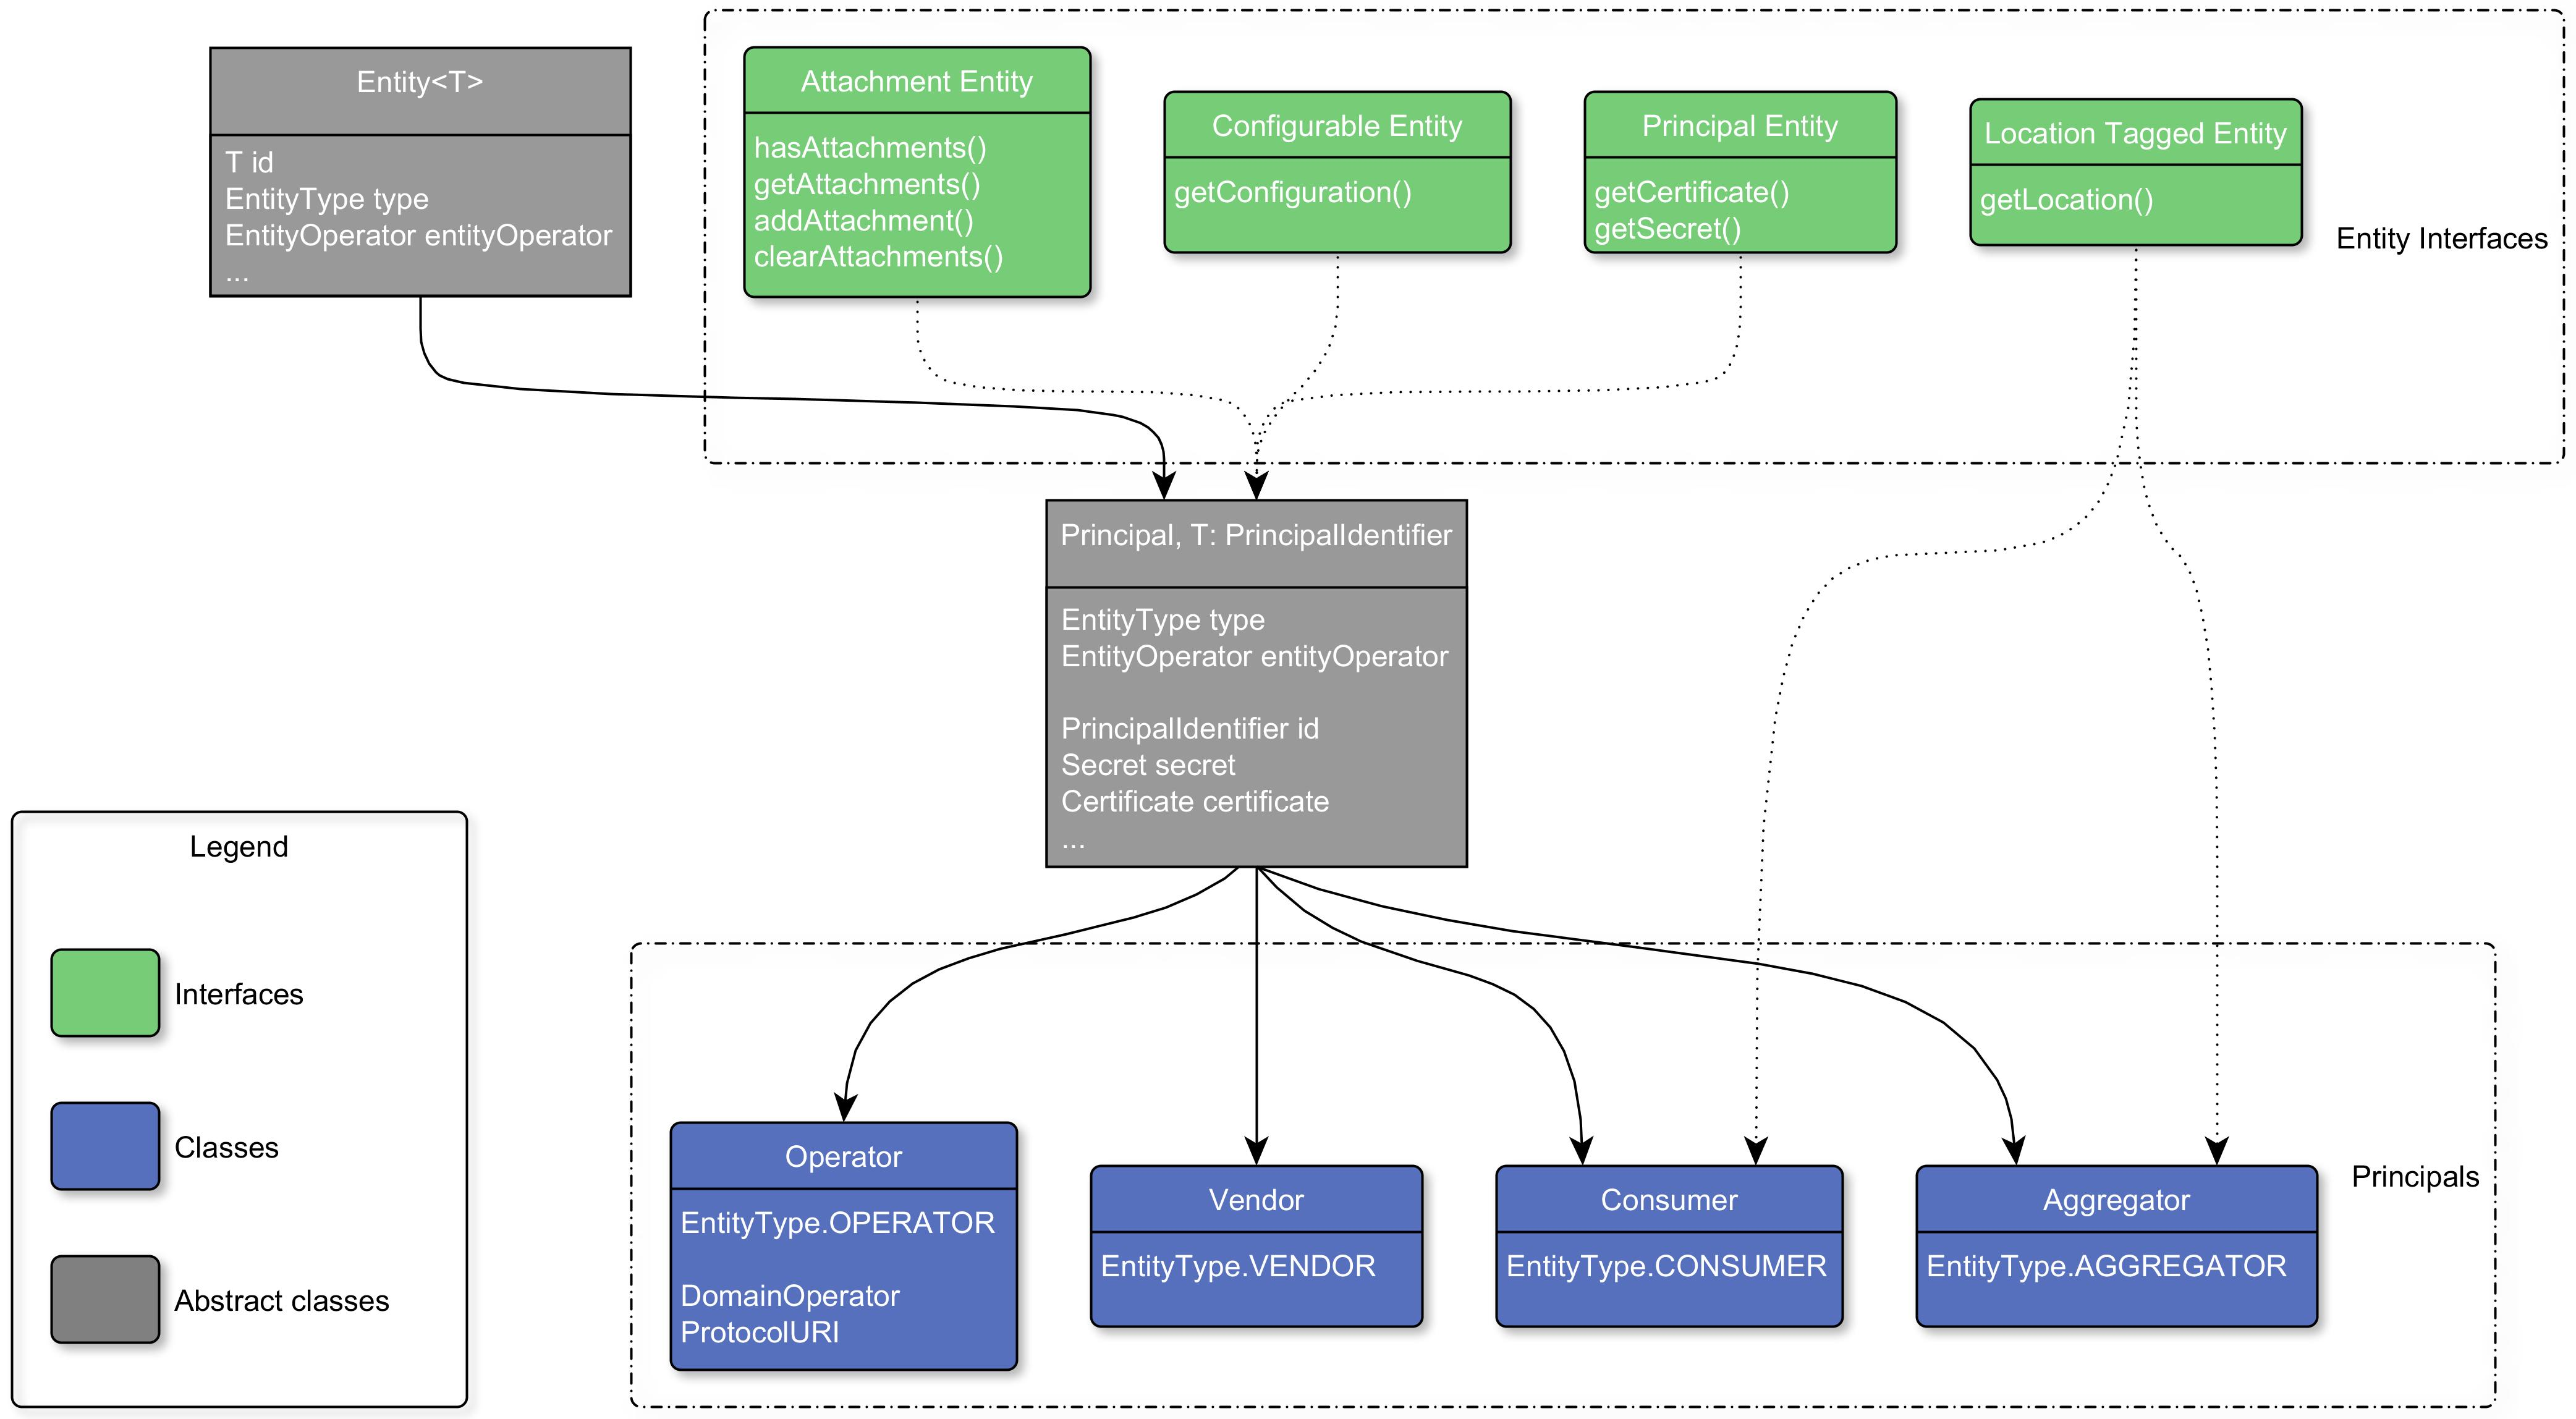
\includegraphics[angle=90,width=0.8\textwidth]{images/principals}
\end{figure}

\subsection{Consumer Profile}
\label{consumer_profile_model}
The consumer profile implementation has been already partially described in the \citetitle{reference_thesis}:
the consumer profile defines a set of software modules and a set of paths between those to enable automatic deployment of a chain of modules. Operations like automatic data format conversion could for example be achieved easily, by adding a converter module between the raw data of the device and the output. 

Such paths of software modules logically always refers to a specific device category (blood pressure, glucose meter, etc). Therefore, the paths are grouped within entries. The consumer profile contains those entries, each bound to a specific device category and describing modules paths. For a specific device category, an entry can be then best described as "a directed acyclic graph, which defines the processing of a data stream".

The same module can be used in several entries, but is deployed only once: it is defined within the scope of the consumer profile. To reflect that, a Node object regrouping both a module and an ID has been introduced. The Nodes are defined in the consumer profile with an unique ID and a unique module, and the different entry paths will then just refer to the corresponding IDs. 
%It must be here also noted that it is not the role of the User Directory to store direct information about devices, like software modules. Instead, information is stored, that is sufficient to retrieve the module, like an identifier (ModuleIdentifier).

Ultimately, the Consumer Profile defines a list of entities who are allowed to read it, as stated in section \ref{03_consumer_profile_authorization}. Only those entities and the EntityOperator can get the profile in order to, for instance deploy automatically a chain of modules.

With this definition, the consumer profile introduced in section 2, with the diabetic glucose meter (see \hyperref[02_consumer_profile_example]{consumer profile example}), could be depicted as in Fig. \ref{fig:consumer_profile_example}. The first entry specifies the data conversion from a proprietary format to a standard CSV format. A second entry is rendered, only for representation purposes.\linebreak

\begin{figure}[!hpbt]
	\centering
	\caption{Consumer Profile Example}
	\label{fig:consumer_profile_example}
	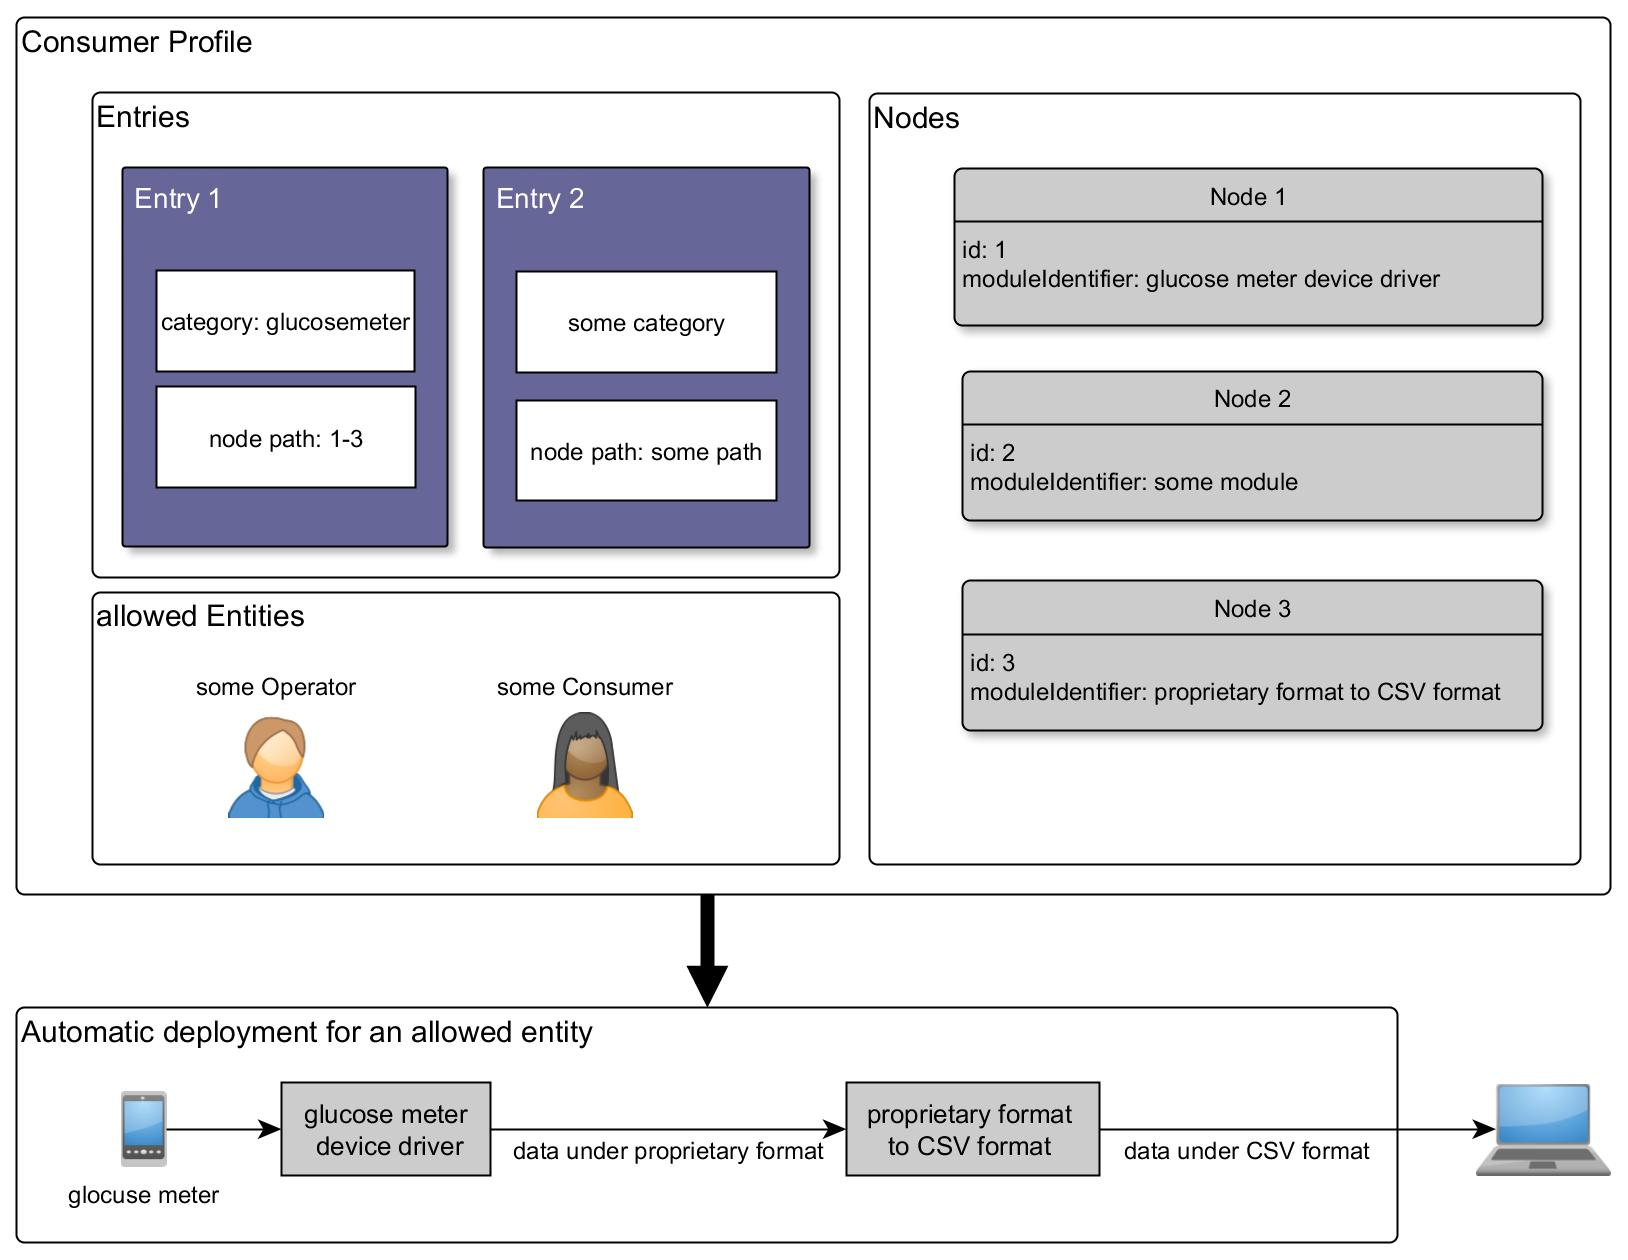
\includegraphics[width=1\textwidth]{images/consumer_profile_example}
\end{figure}

The consumer profile and the consumer profile entries, as they respectively express the consumer's preferences and a deployment scheme, requires to be highly configurable. Moreover, it is conceivable for both to be created, added, updated or removed directly from a user request. For these reasons, both can be regarded as entities of the User Directory.

They extend therefore the generic abstract Entity class and inherit  from the interfaces ConfigurableEntity and AttachmentEntity defined in Tab. \ref{tab:entities_interface} (which means that files or sets of configuration key-value pair can be attached).

\section{Architecture}
The User Directory has been structured to enhance re-usability and modularity, as shown in Fig. \ref{fig:code_struct}. Basically, a few interfaces and abstract classes have been defined that allow any security implementation to be plugged in as module:

\begin{description}
	\item[communication interface]: this is the communication layer of the application. It receives the requests of the clients, performs basic controls like checking authentication, parsing the requests and calling the good logic method with the appropriate arguments..\\
	\item[logic interface]: this interface performs the methods of the authentication and authorization framework defined  in the section \ref{sec:04_framework}. It calls the low-level services and coordinates them to handle any request from the clients.\\
	\item[authentication layer]: handles both type of authentication request, \textit{authenticate} and \textit{delegated authentication}. Implementations of those interfaces performs specific security framework operations, like OpenID Connect, Kerberos, etc..\\
	\item[authorization layer]: since authorization is  performed only for modification or creation of persisted entities (see Tab. \ref{tab:access_control}), an authorization layer is placed on top of the data persistence layer and interfaces with the other layers. It defines the right to create, read, remove or update a persisted entity for any principal. \\
	\item[persistence services] handles any operation of all the persistence systems (at least two, one for the principals and one for the other entities) which enables to create, remove, update or simply get entities of the persistence systems.\\
	\item[session management]: session management is performed in parallel and provides the others component with an authentication context (who is authenticated, etc).
\end{description}


\begin{figure}[hpbt]
	\centering
	\caption{Structure of the project}
	\label{fig:code_struct}
	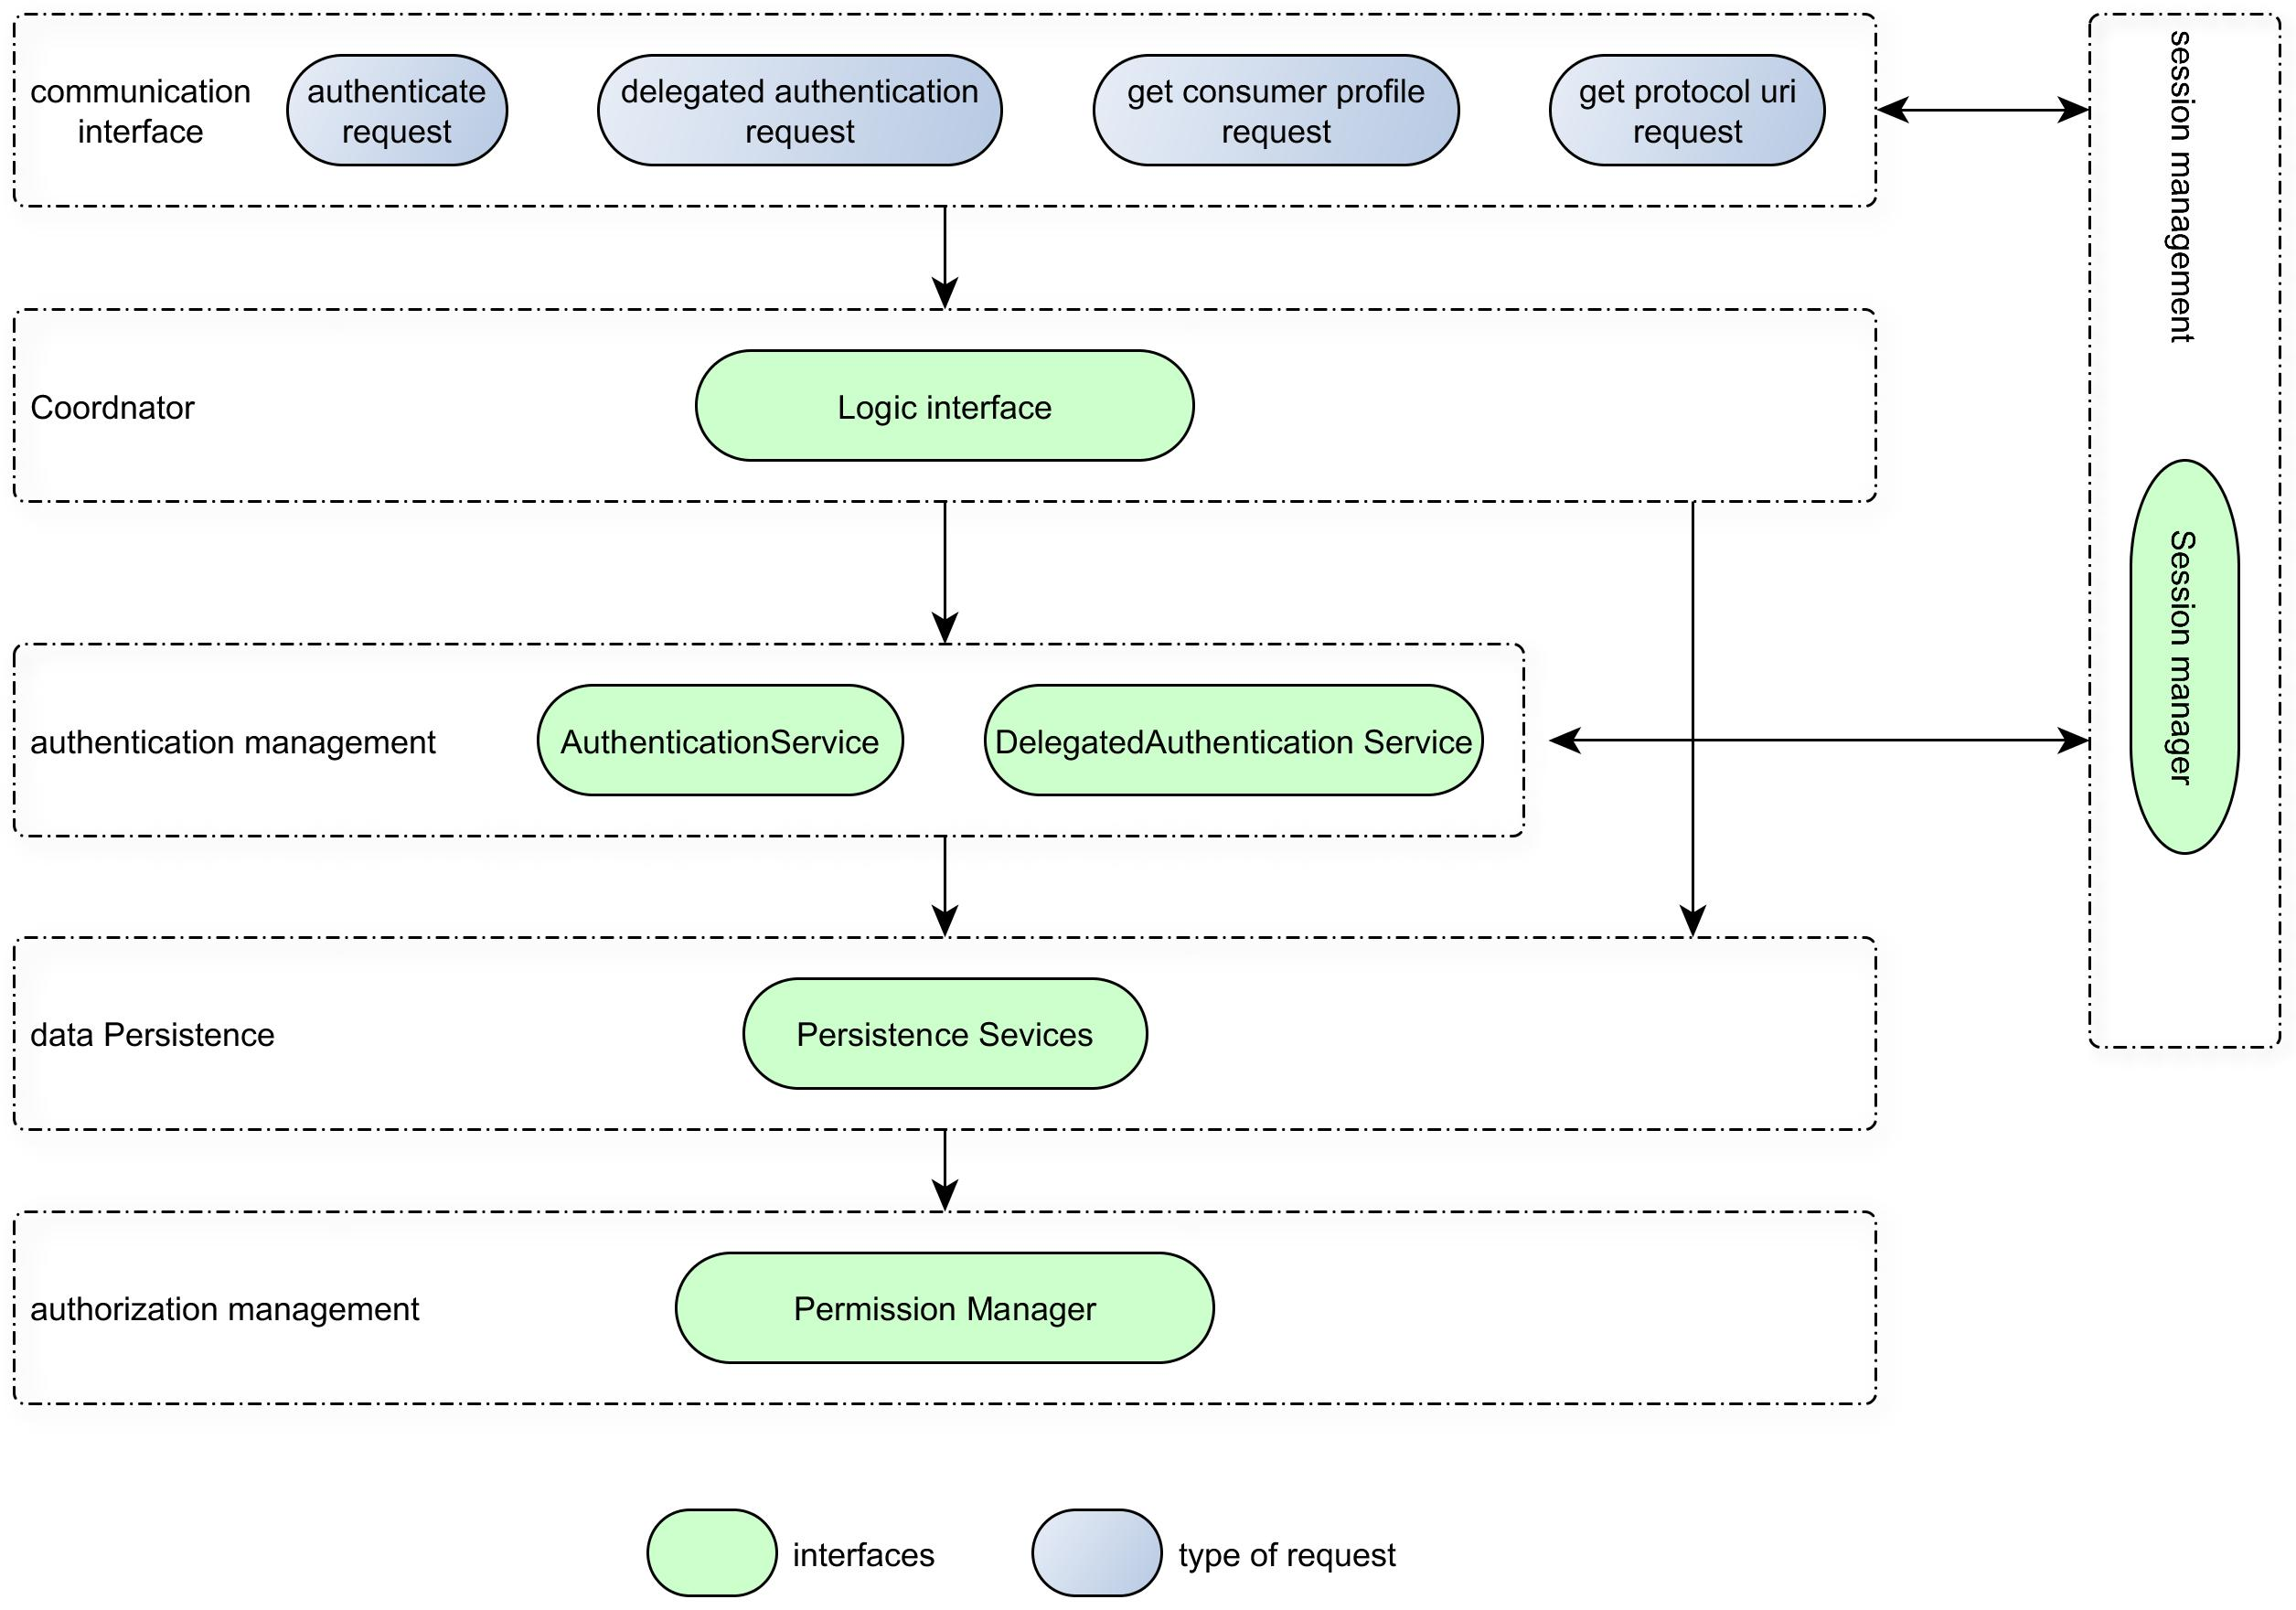
\includegraphics[angle=90,width=0.95\textwidth]{images/code_struct}
\end{figure}

\section{Session Management}
The session manager is the component whose role is to handle every session opened by Principals of the \emph{device cloud}. It creates new sessions and finds or removes existing ones. 

A session must be understood as an authentication context, containing among others the Principal opening the session, the time at which it is opened as well as a unique identifier sessionID. The Principals, when communicating with the server, just have to attach the sessionID. This way, it is authenticated. 

This approach has been preferred to the cookie based one, because combined with TLS/SSL, nobody can access the sessionID without the consent of the Principal. A cookie, in the other hand, has inherent weaknesses since it is not more than a file stored on a hard drive.

Based on the time and sessionID information, the session manager also includes functions to retrieve an opened session from a sessionID and check the validity of a session (if it is not outdated). This way, it enables the other components to check authentication information for any principal.

Most of the security leaks regarding sessions consists in the disclosure of the sessionID. Several weaknesses are known: session fixation (the sessionID of a user is set by the attacker. It can be done for example with server which accepts a new sessionID as HTTP parameter), session hijacking, XSS, session prediction (sessionID easy to guess) or weak sessionID storage.

The use of TLS/SSL and the non-use of cookies defeats any session hijacking attempts (sniffing cannot be done). Combined with a websocket communication and the fact that the session does not create new sessions based on request parameters, it also prevents session fixation. The java websocket architecture also erases any possibility of XSS attack (no scripting language is ever ran).
Session prediction can be avoided by choosing a sufficient minimal length. In this case, the session ID contains at least 20 characters. Finally, a weak session storage can compromise the session IDs if an attacker can access the storage. The implementation keeps the ids in the java virtual machine and never store them on the hard drive. Thus, this weakness is also handled.

Nevertheless, with enough time, any cryptographic system can be broken, and the sessionID stolen. Therefore, the validity time of a session has been set as configurable property. This validity time should be chosen wisely. In the implemented solution, the sessions last for 1 hour.


\section{Persistence}

\subsection{Data Access Object pattern}
Each persistence service has been build with the same structure. This structure corresponds to a Data Access Object (DAO) design pattern. This pattern is now a widely accepted mechanism to abstract away the details of persistence in an application. Instead of having the domain logic communicate directly with the persistence system (database, file system, web service, etc), the domain logic speaks to a DAO layer instead. This DAO layer then communicates with the underlying persistence system or service.

The advantage of using such a DAO layer is that if the underlying persistence system is changed, only the DAO layer should be adapted. The entity classes that are persisted (in this case the Principals and the consumer profile), for example, can be kept. 

Thus, the persistence layer contains a service per type of entity. The CRUD method can then be called from this service. A read operation on a Consumer would then be achieved by the following call (it is assumed that the Session Management Layer provided a so-called \textit{context}):

\lstset{language=Java}
\begin{lstlisting}
	PersistenceManager.getPersistenceService(EntityType.CONSUMER).get(consumerID, context)
\end{lstlisting}


It should also be  remembered that entities can inherit from the AttachmentEntity interface, as shown in Tab. \ref{tab:entities_interface}. That means that files can be attached to an entity, and must be thus stored when the entity is persisted. 

Therefore, every persistence service adds a file-system storage mechanism to its standard storage mechanism (LDAP, database, etc).

\subsection{Principal Persistence}

As mentioned earlier, persisting principals within a Domain can be done either with a dedicated database, or with an existing IAM solution.The Domain Operator will create new principals and verify the validity of incoming connections with this persistence system. For security purposes, the Domain Operator must be the only entity with access to this persistence system.

For this thesis, LDAP-based and dedicated database solutions have been analyzed. 

In fact, there are not many fundamental differences between the two approaches, since most LDAP implementations are based on a backend database. However, one could sum up the plus and cons of both as depicted in Tab. \ref{tab:ldap_db}:

\begin{table}[h]
	\caption{A Comparison of LDAP and database solutions}
	\centering
	\label{tab:ldap_db}
	\begin{tabular}{|c|l|l|}
		\cline{2-3}
		\multicolumn{1}{c|}{} & 
		\multicolumn{1}{|c|}{\cellcolor{Gray}\textcolor{white}{\textbf{Database}}} & 
		\multicolumn{1}{|c|}{\cellcolor{Gray}\textcolor{white}{\textbf{LDAP}}} \\
		\hline
		\cellcolor{Gray}\textcolor{white}{\textbf{Plus}} &
		\pbox{0.4\linewidth}{
			\vspace{0.5em}
			\textbullet \quad support for transaction \\
			\textbullet \quad simpler
		} & 
		\pbox{0.4\linewidth}{
			\vspace{0.5em}
			\textbullet \quad very fast for read operations \\
			\textbullet \quad support for different authentication methods \\
			\textbullet \quad designed with security in mind
		} \\
		\hline
		\cellcolor{Gray}\textcolor{white}{\textbf{Cons}} &
		\pbox{0.4\linewidth}{
			\vspace{0.5em}
			\textbullet \quad offers a broader surface attack \\
		} & 
		\pbox{0.4\linewidth}{
			\vspace{0.5em}
			\textbullet \quad slow for write operations \\
			\textbullet \quad no transaction support \\
			\textbullet \quad heavier configuration
		} \\
		\hline
	\end{tabular}
\end{table}

The transaction support is a big deal in many systems, as it is possible to rollback when an error occurs. But in the authentication framework, where only authentication must be performed, few operations are needed and none of them require transactions. Indeed, those operations only count a \textit{read} operation and a \textit{compare} operation (for passwords), which is similar to a read operation. Besides, concurrent operations are unlikely to happen since the persistence system is designed to be used by only one user, the Domain Operator.

Another key decision factor here was the security considerations. The LDAP implementations are before all designed for authentication, and thus have a more robust architecture in the sense that they offer support for various security protocols and methods. In addition, a LDAP-based approach separates the data from the authentication, which allows for a better organization and offers a smaller attack surface.

Hence, a LDAP-based approach has been chosen.

\subsection{LDAP implementation}

A LDAP (Lightweight Directory Access Protocol) was originally a protocol to access and maintain directory information services. It has evolved to become a norm, including a data model, a naming model, a functional model based on the protocol, a security model and a replication model.

The LDAP data model defines a hierarchical object tree structure, where every object has a RDN (relative distinguished name). The RDN is a set of key value pair, which is unique in the  object's branch (at the same level of the branch). An object can then be uniquely identified within the whole tree by concatenating its RDN with its ancestors RDNs. This is the so-called distinguished name (DN). The objects composition (structure and attributes) are defined by schemes, which can be either standard, default or custom ones.

The LDAP tree, rendered in Fig \ref{ldap_tree} has been created with the use a custom scheme. The earlier defines standard element like organization (here, the TU Berlin) or organizational unit. The latter defines the following 4 classes: Operator, Vendor, Aggregator and Consumer as well as their attributes. The structure of the tree follows then simply the underlying logic: all above-listed principals belong to their organizational unit (customers, etc) defined by the standard scheme, and constitute in turn the User Directory.

To enhance re-usability, the tree has also as root element an organization (like TU Berlin) and a domain name, in this case userdirectory.devicecloud. Those two objects are also defined by the standard scheme. In the end, a Consumer will be identified by the following Distinguished Name:

\quad \quad \textit{entityID=consumerID, ou=consumers, o=TU Berlin, dc=userdirectory, dc=devicecloud}

The LDAP server used is an OpenLDAP Server, mainly because it offers a good documentation and worldwide commercial support. It is also highly configurable. The configuration might be easier with other LDAP servers, like ApacheDS or OpenDJ, but is also shipped with client applications (respectively Apache Directory Studio and OpenAM), with which users and groups can be  managed more easily. Since the Principals of the \emph{device cloud} are defined with a custom scheme, those features are not required.

Finally, the security measures defined in \ref{LDAP_security} have also been implemented. One can connect to the LDAP Server without use TLS/SSL, but any action requires to be authenticated, and the only way to authenticate has been configured as SSL Certificate authentication.

The configuration of the LDAP might be tedious, because it involves many different steps (creation of LDAP, configuring basic properties like communication port or logging, adding custom schemes, configuring SSL, setting the privileges to the legitimate entities, restraining the rights of all others, etc) and because the error messages of the LDAP are not very descriptive. 

Consequently, a docker file has been created, that allows for a quick deployment of a working LDAP server. Basic properties like communication port or IP of the User Directory machine must be first set in the docker file, a simple docker run then deploys the LDAP server.


\begin{figure}[tbhp]
	\centering
	\caption{Structure of the LDAP tree}
	\label{ldap_tree}
	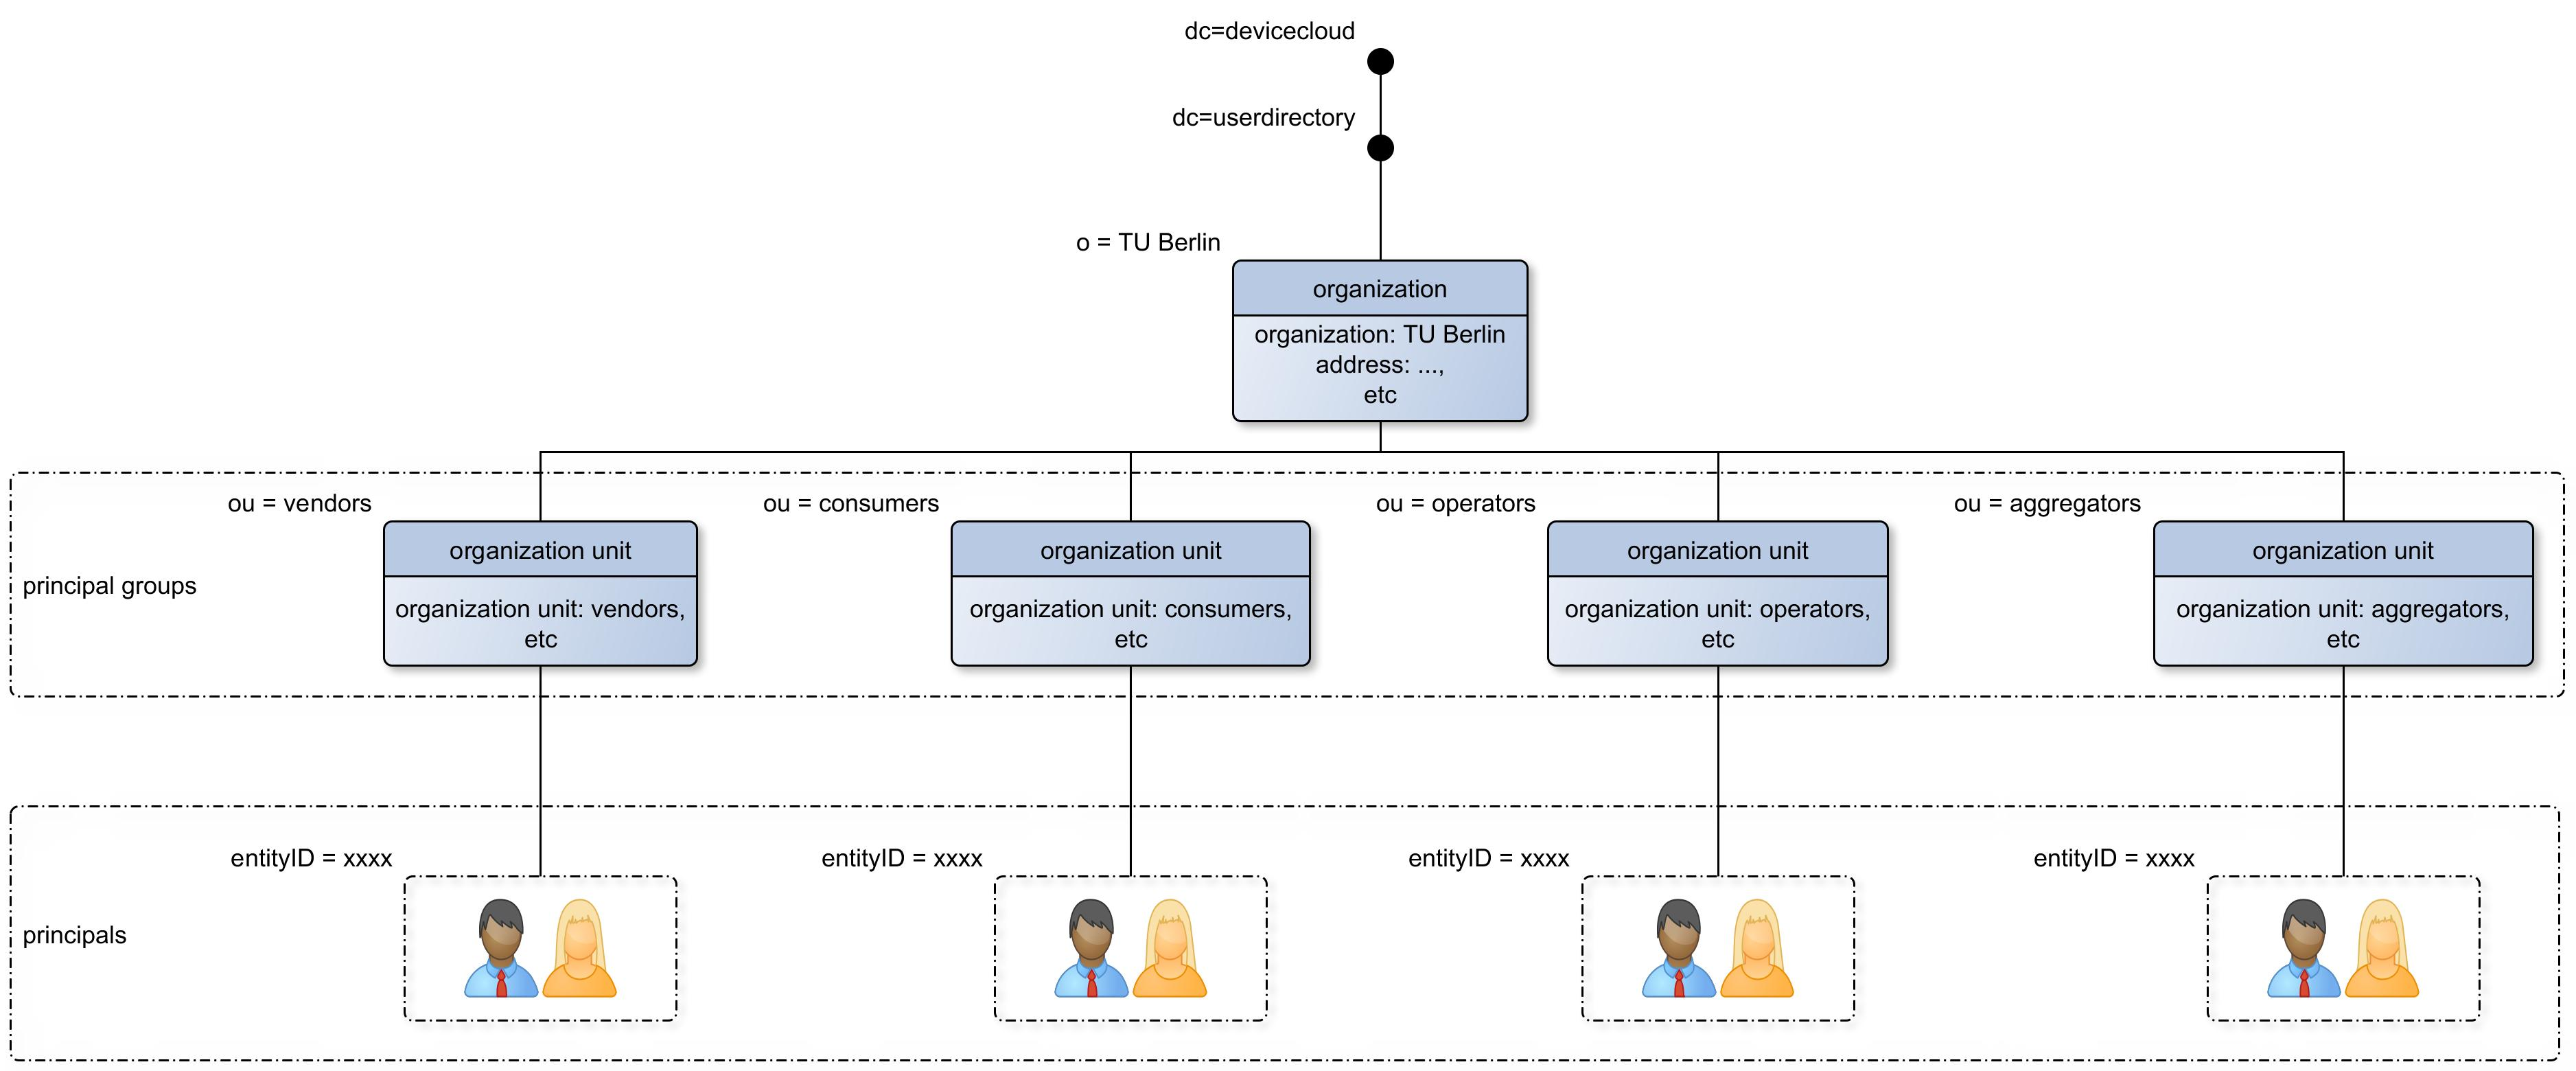
\includegraphics[angle=90,height=\textheight]{images/ldap_tree}
\end{figure}

\subsection{Consumer Profile persistence}

As required by the design, a separated database has also been used for the Consumer Profile and its components (the entries and nodes, defined in section \ref{consumer_profile_model}). The database used is a HyperSQL in-memory database (HSQLDB), based on the previous work done on the \emph{device cloud}. 

This database has been protected by a username/password pair that only the domain running the database should possess, as required in section \ref{sec:03_database}. However, since the in-memory database was used essentially for testing purposes, no further security measures were implemented.

\section{Testing}
This sections explains how the User Directory has been tested. By User Directory, the result of the four methods \textit{authenticatePrincipal}, \textit{authenticatePrincipalForThirdParty}, \textit{getConsumerProfile} and \textit{getProtocolUris} is meant (see \hyperref[interface_methods]{methods}).

Testing the authentication framework can not just be done with unit tests, since an end-to-end connection must be established (an Principal authenticates to its IdP for example, over a SSL secured channel). Every test must therefore have its own configuration, with certificates, private keys, etc.

The workflow of the direct and delegated authentication testing logic, on which the conducted tests are based, is rendered in Fig. \ref{fig:tests_1}: there are for example two possibilities for the authentication to fail: either a bad certificate or bad request parameters. A certificate is considered not valid when it is not signed by the correct CA, or when the information it contains is false (it contains among other the ID of the entity using it). 

This leads to the creation of $ 3 \times 4 = 12 $ certificates and public/private key pairs only for the principals (1 valid and 2 false for 4 types of principals: Consumer, Aggregator, Vendor and Operator). When considering also IdPs and clients, 8 more certificates and key pairs are required. 

Once the configuration done, every test has been successfully performed. It can be thus concluded that the SSL environment and the LDAP (technologies on which relies the authentication) have been correctly configured and that the authentication methods behave as expected. 

Once the authentication methods had been tested, the configuration for the Get Protocol URI and Get Consumer Profile was already set up. Thus, the specifications given in Tab. \ref{tab:access_control} were verified more easily.

\begin{figure}[!tbh]
	\centering
	\subfloat[direct authentication testing structure][direct authentication testing structure]{
		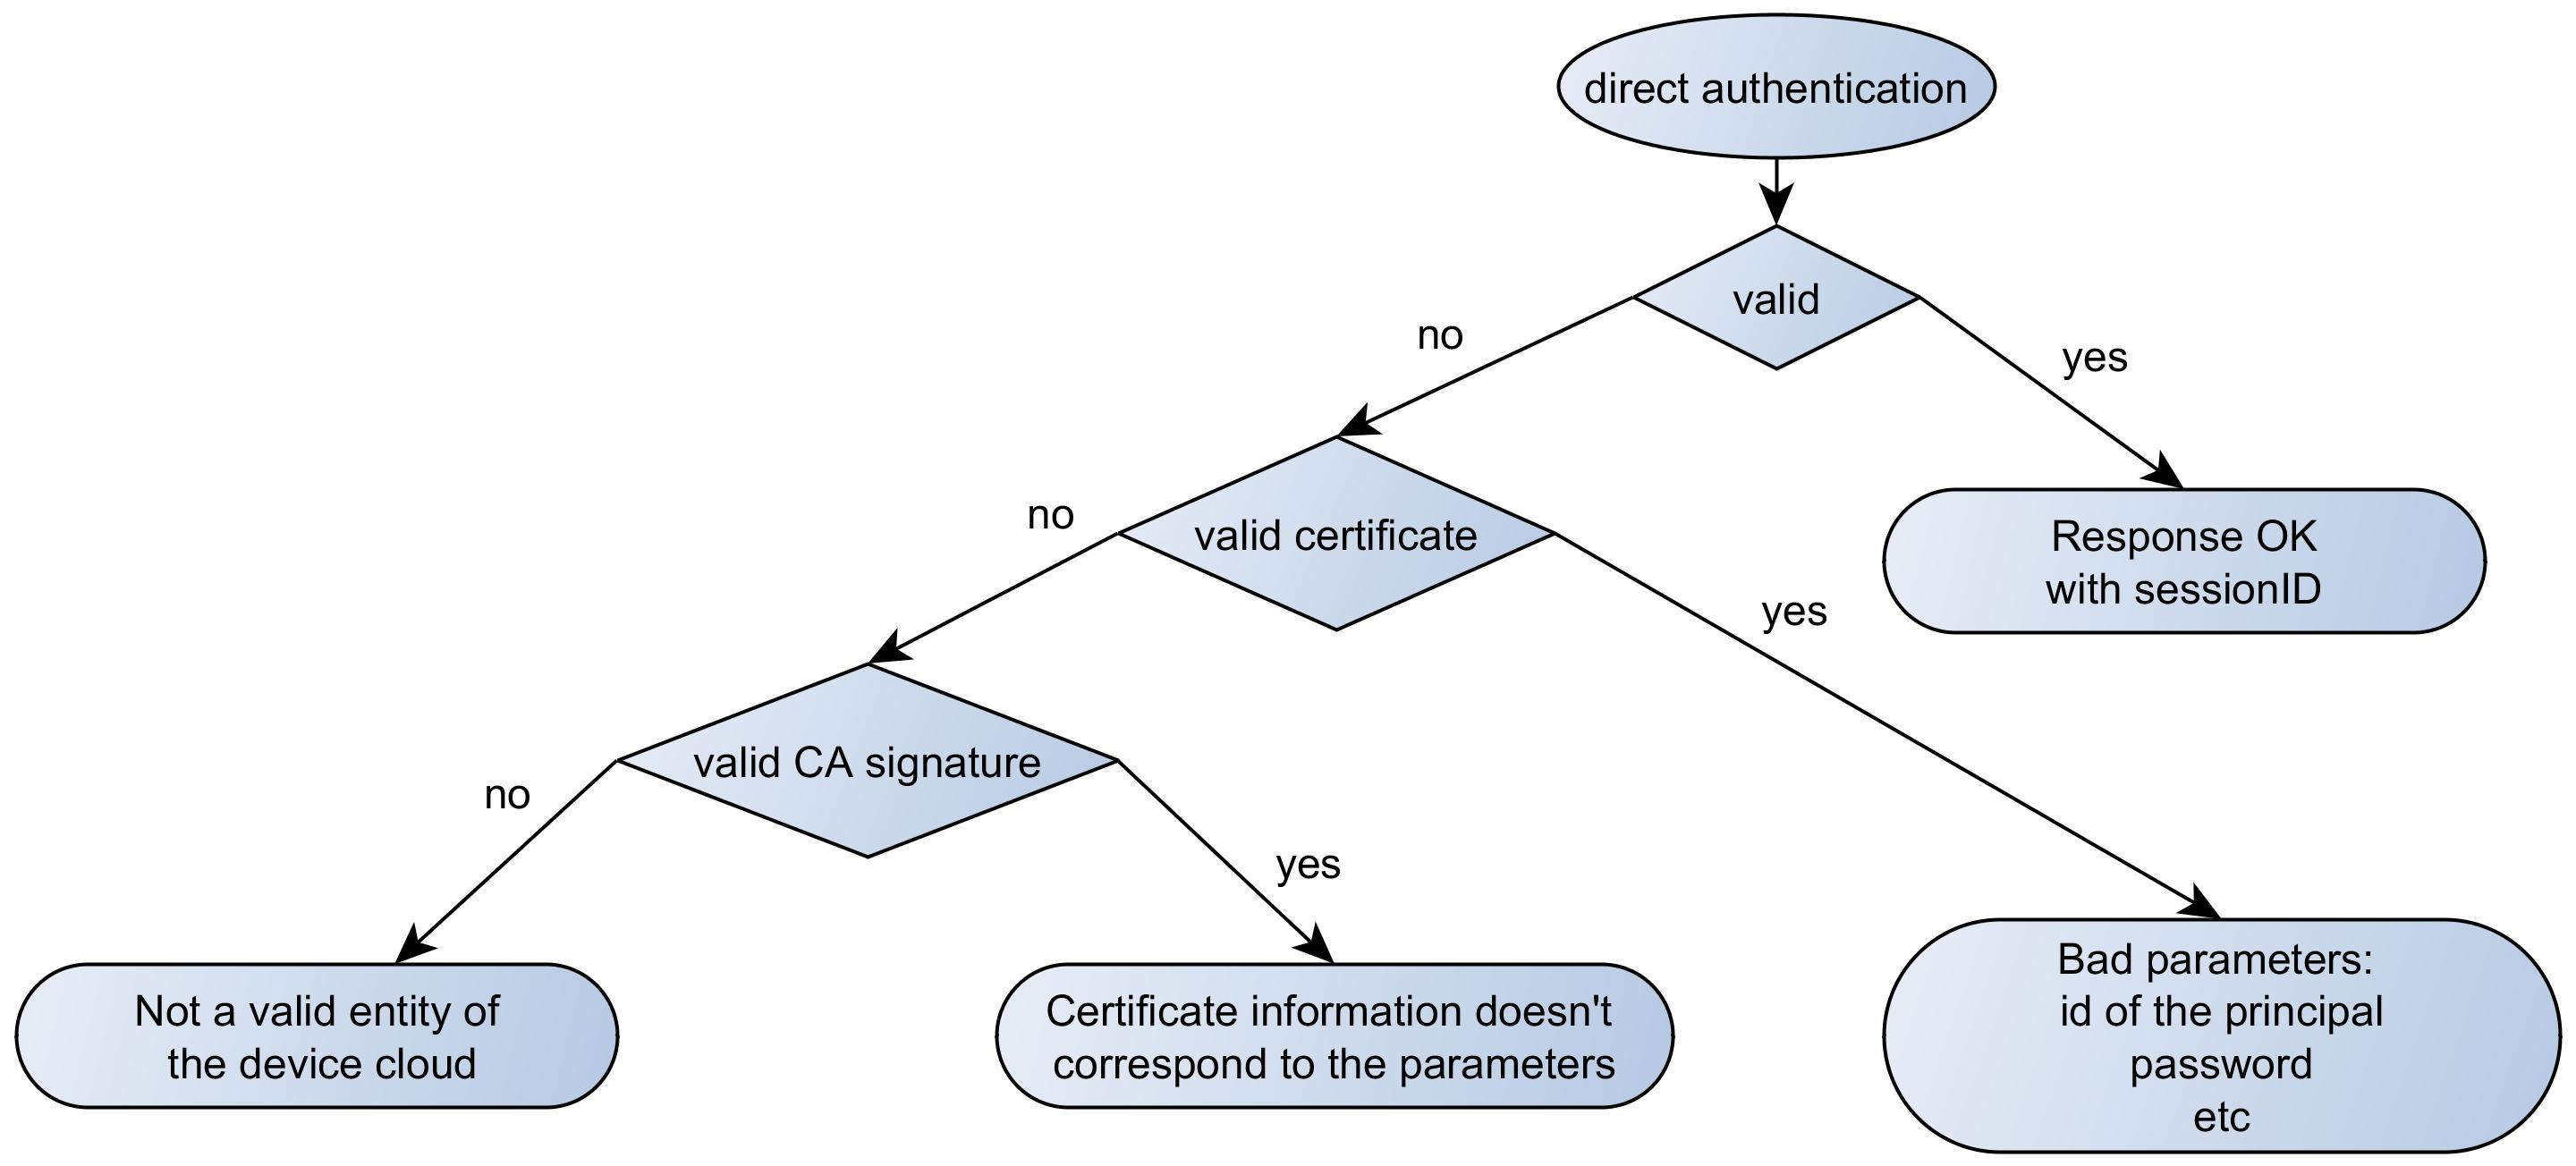
\includegraphics[width=\textwidth]{images/tests}
		\label{fig:tests_1}}
	\qquad
	\subfloat[delegated authentication testing structure][delegated authentication testing structure]{
		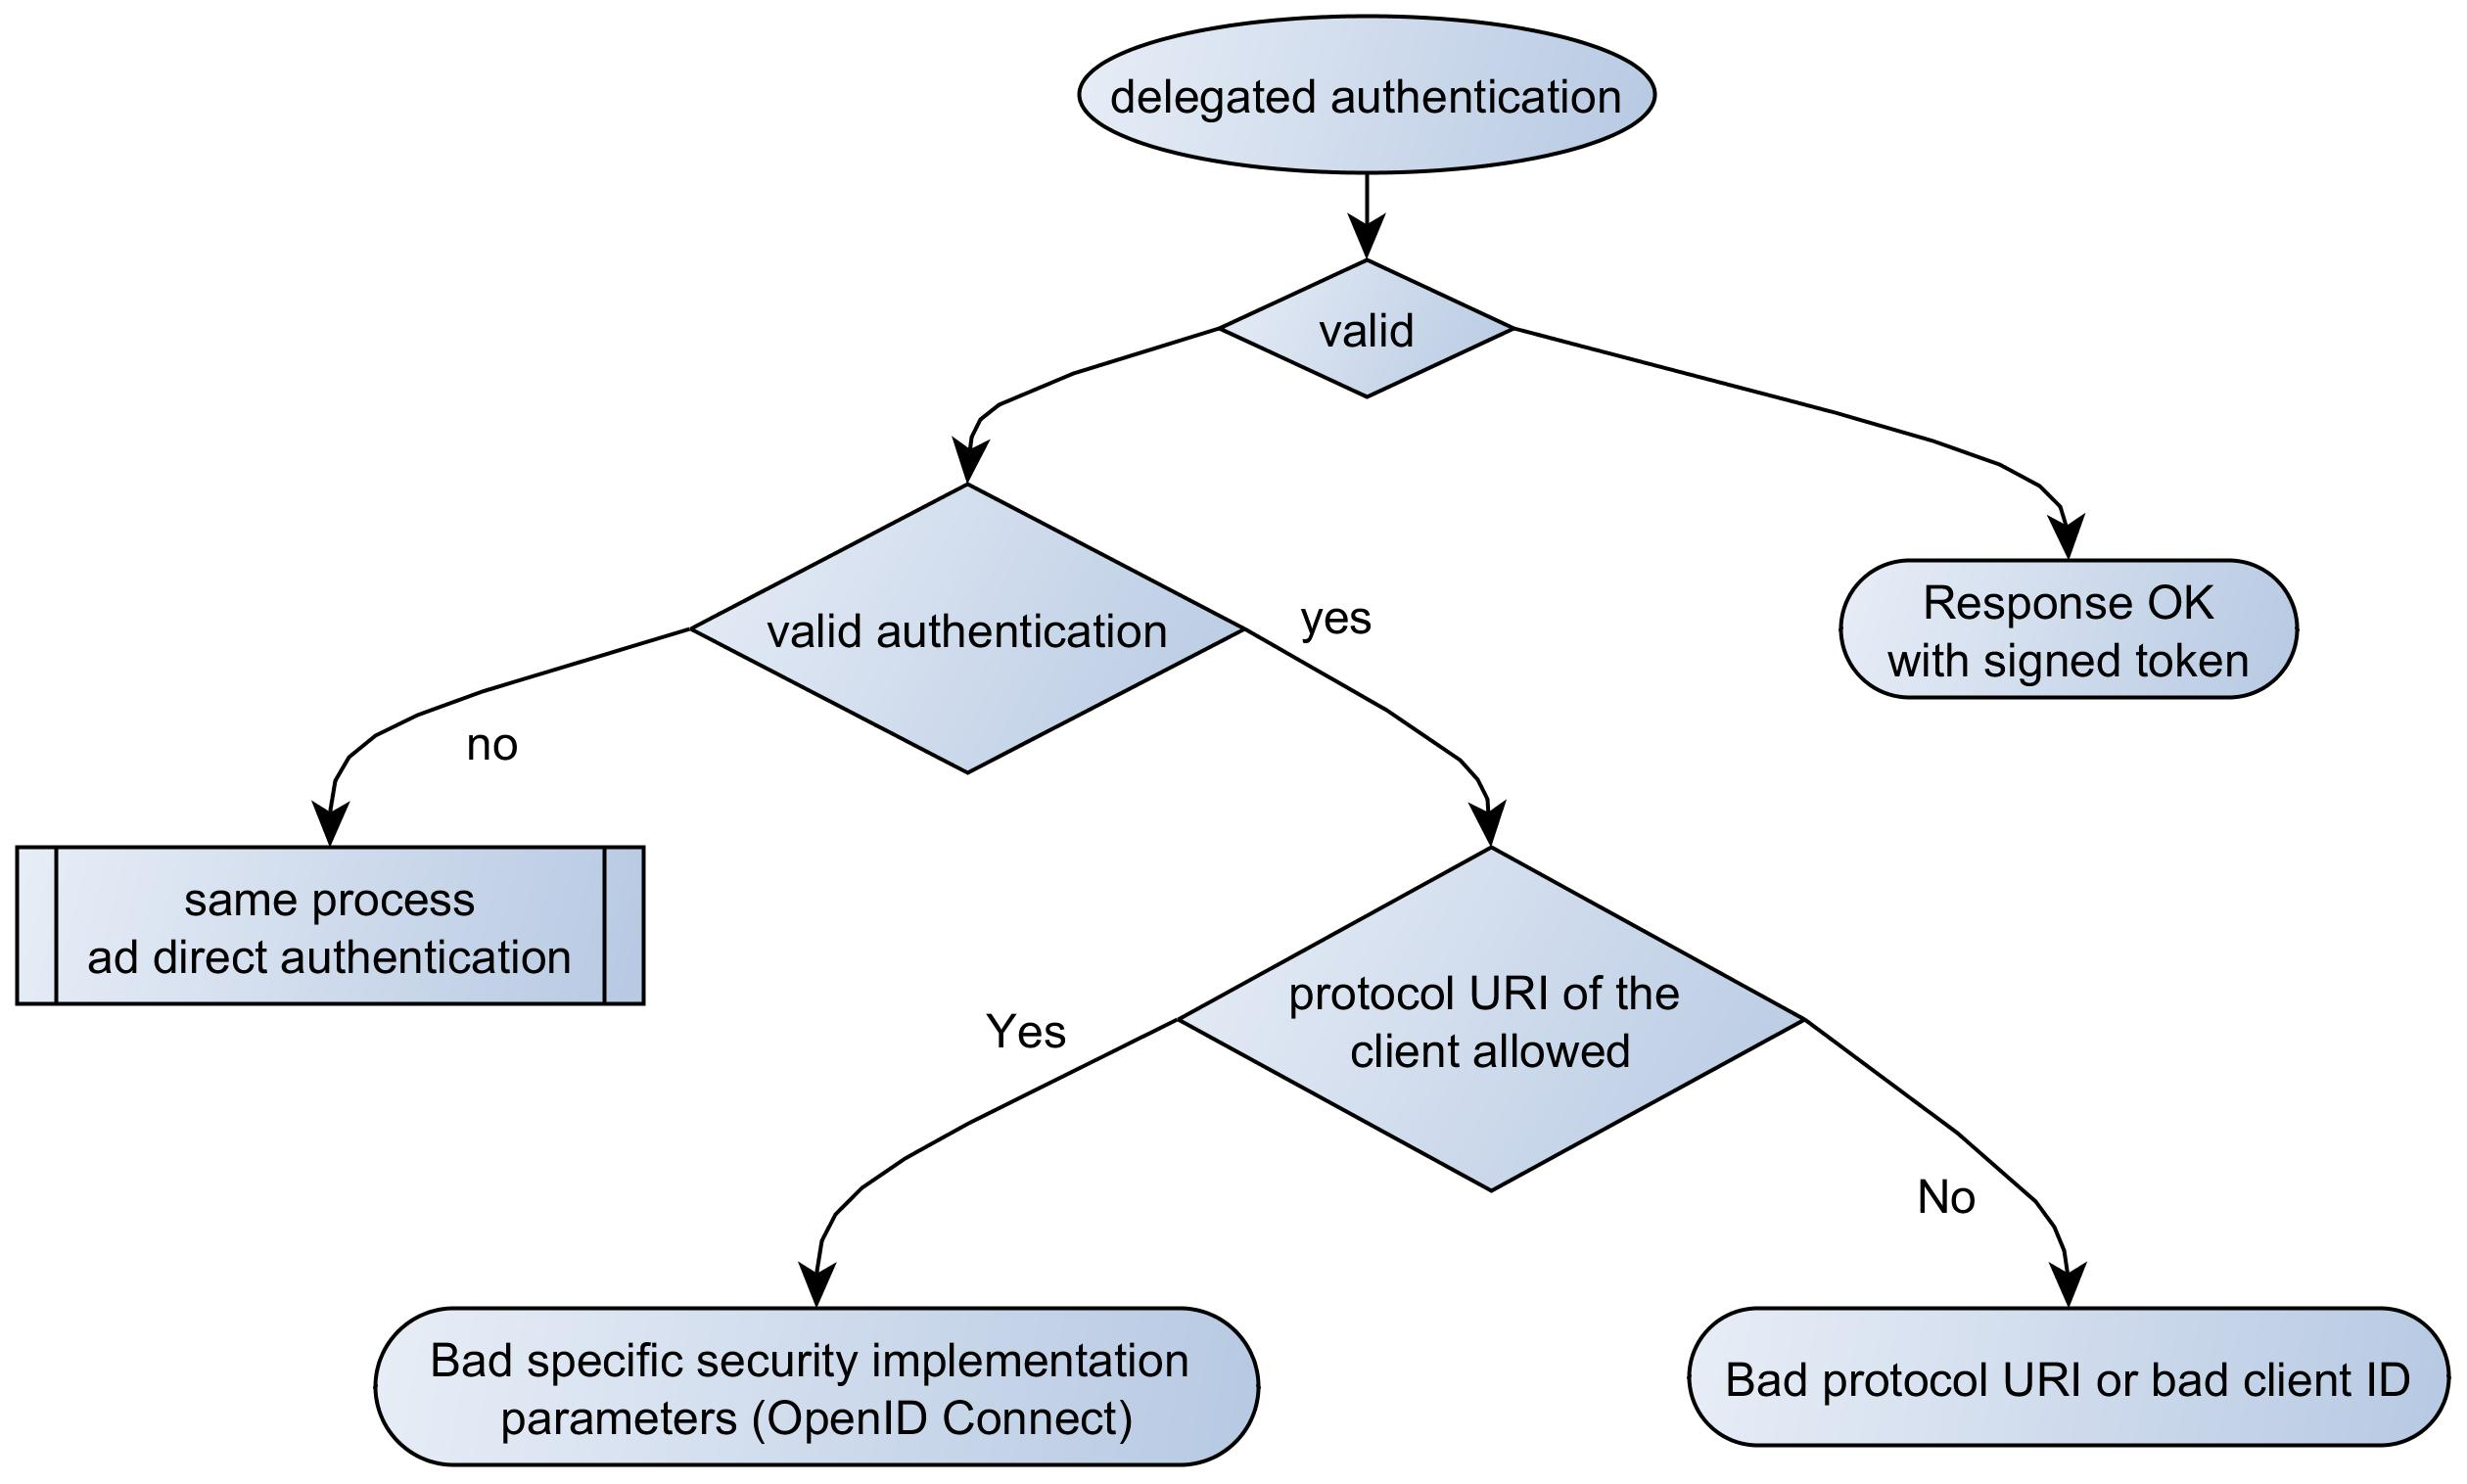
\includegraphics[width=\textwidth]{images/tests_2}
		\label{fig:tests_2}}
	\caption{Tests structure}
	\label{fig:tests}
\end{figure}



